\documentclass[tikz]{standalone}
\usepackage{tikz}
\usetikzlibrary{positioning, graphs}
\usetikzlibrary{graphs.standard}
\begin{document}
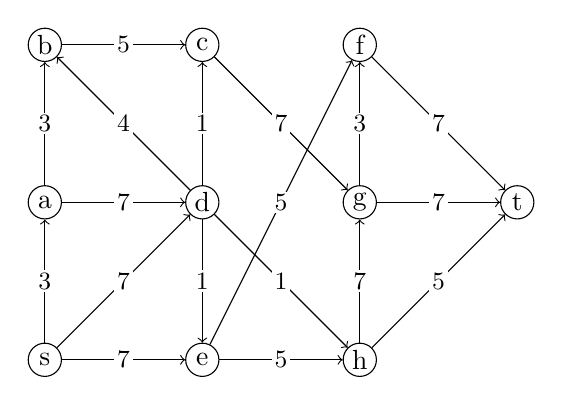
\begin{tikzpicture}
\begin{scope}
		[vertex/.style={draw,circle,inner sep = 0em, minimum size = 1.2em},
		 edgelabel/.style = {fill = white, inner sep = 0.1em, font=\small}]
		\node[vertex] (b) at (0,0) {b};
		\node[vertex] (c) at (2,0) {c};
		\node[vertex] (f) at (4,0) {f};
		\node[vertex] (a) at (0,-2) {a};
		\node[vertex] (d) at (2,-2) {d};
		\node[vertex] (g) at (4,-2) {g};
		\node[vertex] (t) at (6,-2) {t};
		\node[vertex] (s) at (0,-4) {s};
		\node[vertex] (e) at (2,-4) {e};
		\node[vertex] (h) at (4,-4) {h};
		
		\draw[->] (s) to node[edgelabel] {$3$} (a);
		\draw[->] (s) to node[edgelabel] {$7$} (d);
		\draw[->] (s) to node[edgelabel] {$7$} (e);
		\draw[->] (a) to node[edgelabel] {$3$} (b);
		\draw[->] (a) to node[edgelabel] {$7$} (d);
		\draw[->] (b) to node[edgelabel] {$5$} (c);
		\draw[->] (c) to node[edgelabel] {$7$} (g);
		\draw[->] (d) to node[edgelabel] {$4$} (b);
		\draw[->] (d) to node[edgelabel] {$1$} (c);
		\draw[->] (d) to node[edgelabel] {$1$} (e);
		\draw[->] (d) to node[edgelabel] {$1$} (h);
		\draw[->] (e) to node[edgelabel] {$5$} (f);
		\draw[->] (e) to node[edgelabel] {$5$} (h);
		\draw[->] (f) to node[edgelabel] {$7$} (t);
		\draw[->] (g) to node[edgelabel] {$3$} (f);
		\draw[->] (g) to node[edgelabel] {$7$} (t);
		\draw[->] (h) to node[edgelabel] {$7$} (g);
		\draw[->] (h) to node[edgelabel] {$5$} (t);
\end{scope}
\end{tikzpicture}
\end{document}